\documentclass[a4paper, 11pt]{article}
\usepackage[T1]{fontenc}
\usepackage{lmodern}
\usepackage{amsmath}
\usepackage{amssymb}
\usepackage[pdftex]{graphicx}
\usepackage{url}

\title{Supernovae type Ia as standard candles}
\author{A concept for a school lesson\\\\HERAEUS Summer school, Group 3}
\date{26.08.-03.09.2017}

\begin{document}
  \maketitle
  \tableofcontents
  \newpage
  \section{distance measurements}
    \begin{figure}
      \label{ladder}
      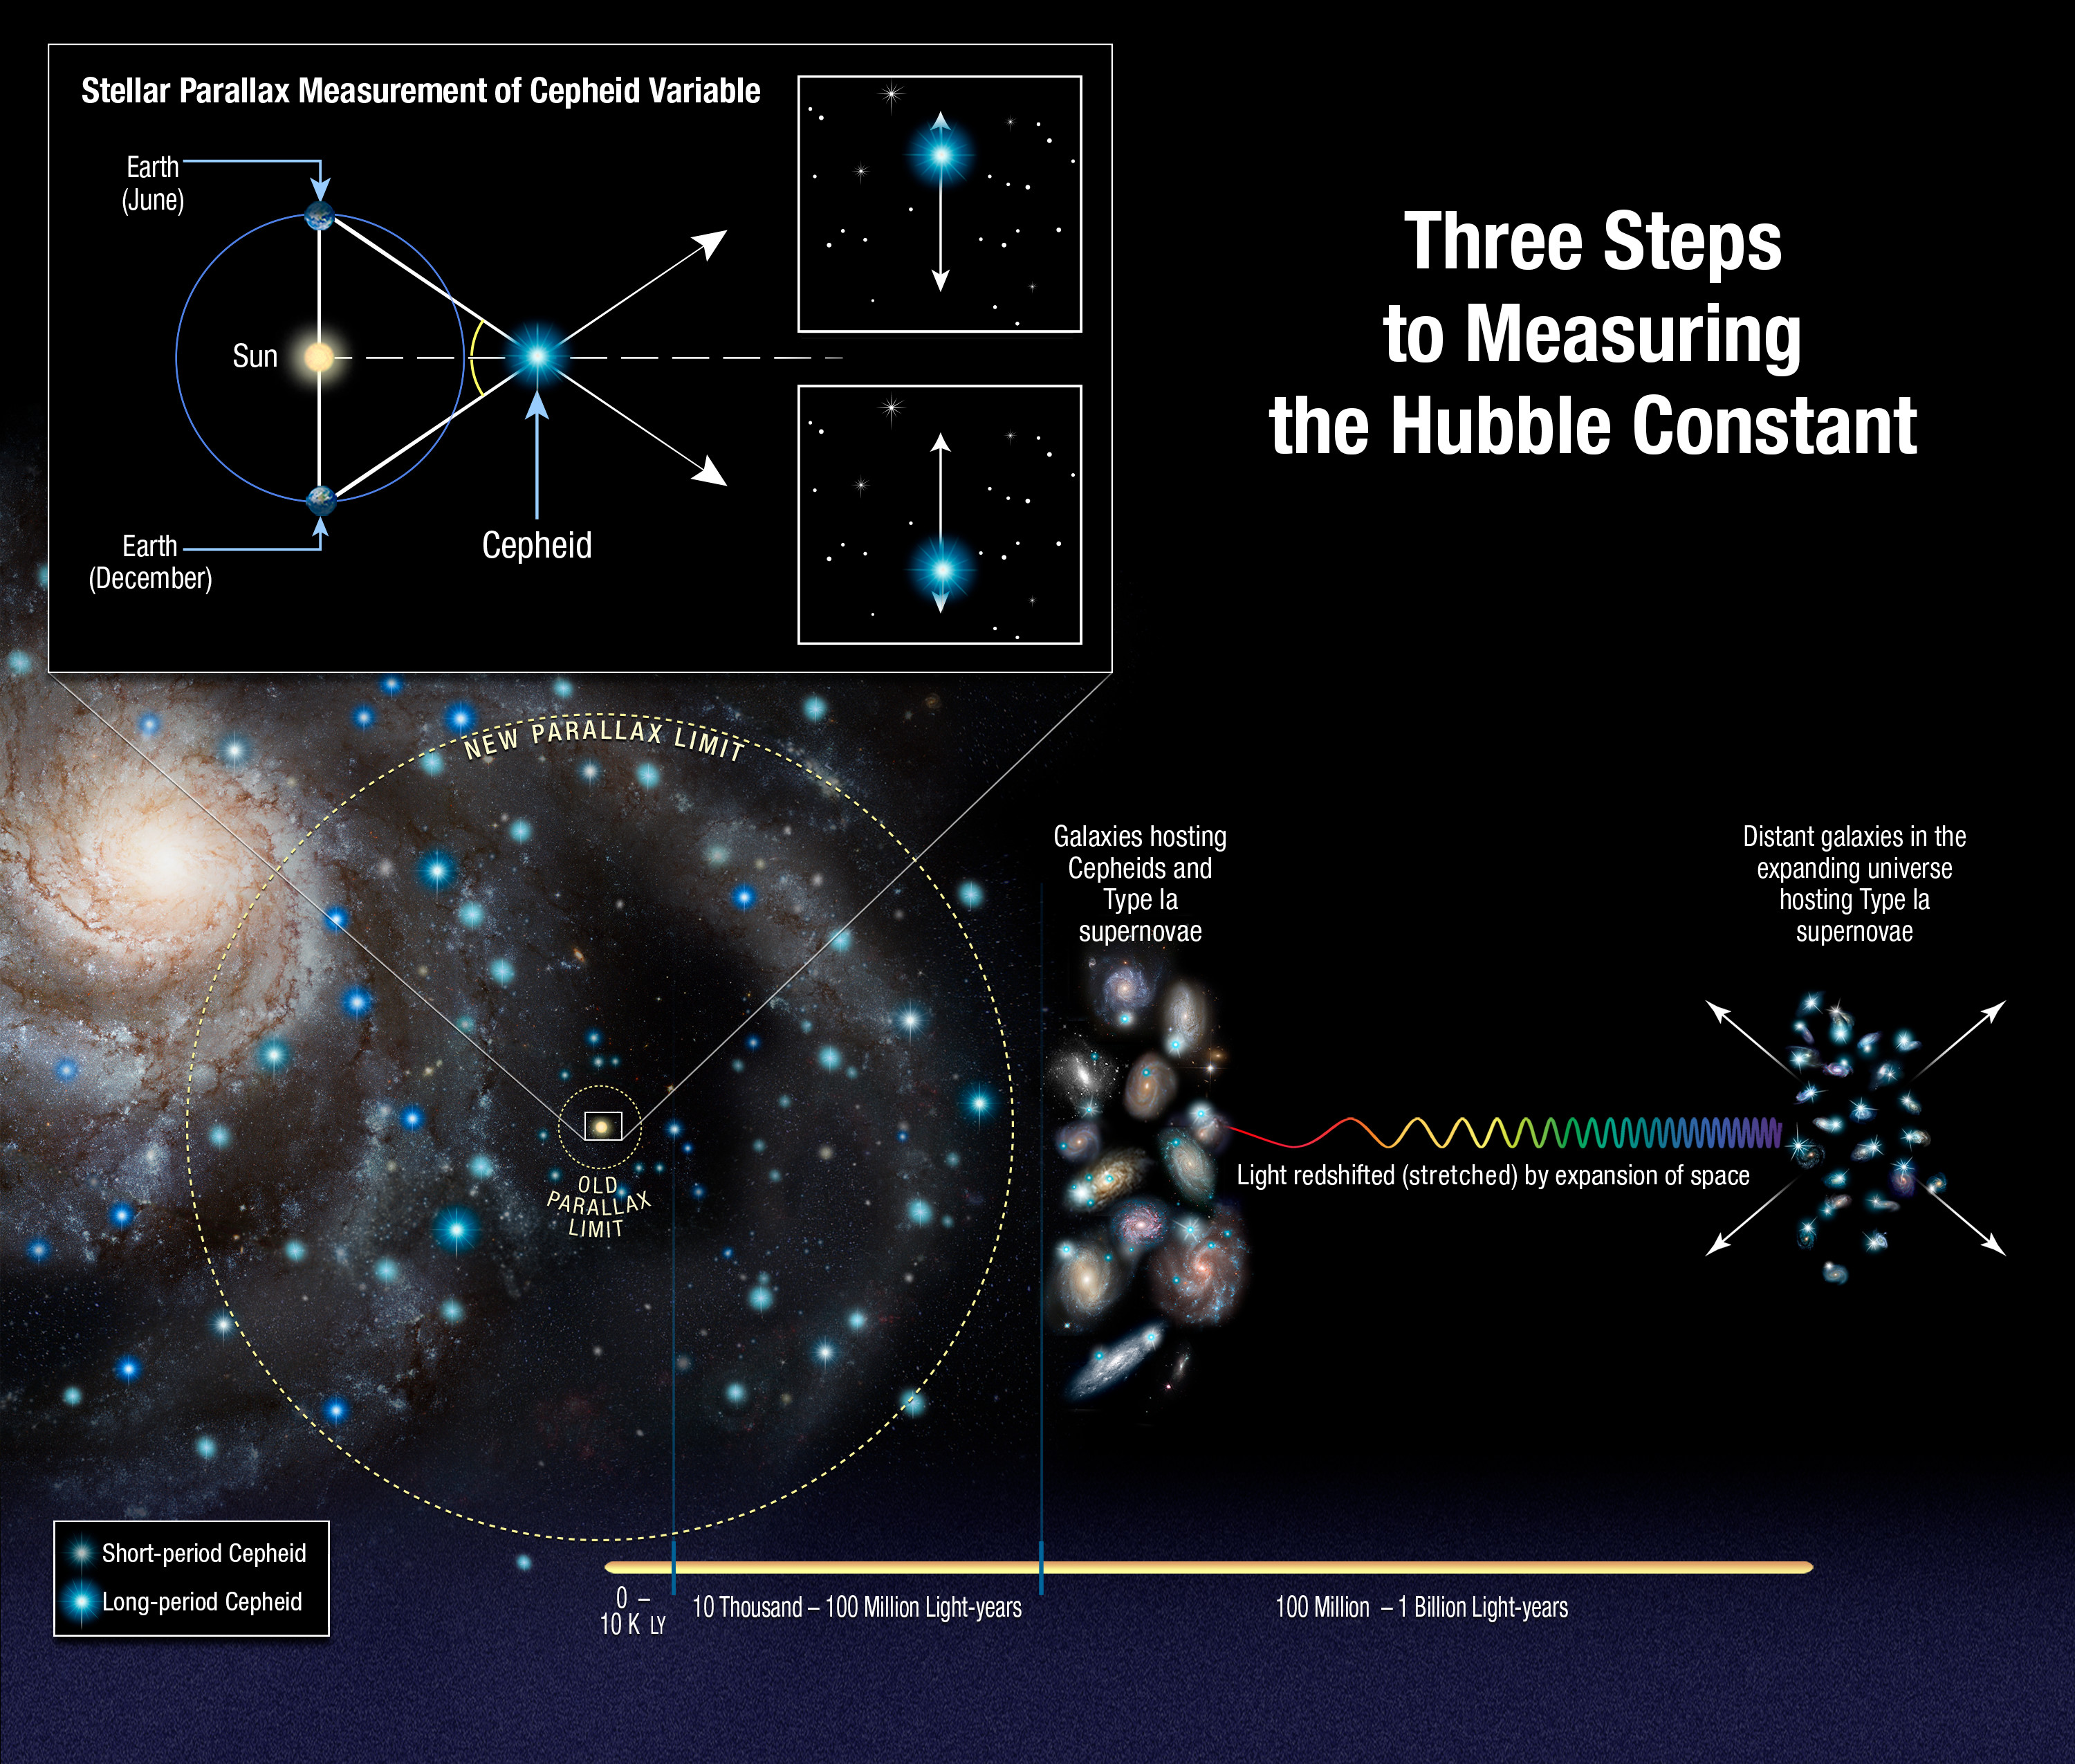
\includegraphics[width=\textwidth]{distanceladder.jpg}
      \caption{distance ladder showing different measurement methods and their limits. \hfill Image: NASA, ESA, A. Feild (STScI), and A. Riess (STScI/JHU)}
    \end{figure}
    \begin{itemize}
      \item restricted via range of applicability (see Figure \ref{ladder})
    \end{itemize}
    \subsection{parallaxes}
      \begin{itemize}
        \item e.g. orbital motion of the earth
        \item mathematical relation $r\sim\frac1p$
        \item $D\simeq\frac{1\,\mathrm{AU}}{p}$
        \item definition of the parsec ($"1\,\mathrm{pc}={1''}^{-1}"$)
        \item range of validity up to $200\,\mathrm{pc}$
      \end{itemize}
    \subsection{photometry}
      \begin{itemize}
        \item star's luminosity decreases with the distance:
          \begin{itemize}
            \item $I=\frac{L}{4\pi r^2}$
          \end{itemize}
        \item comparison of apparent and absolute magnitude yields the distance
      \end{itemize}
      \subsubsection{\textsc{Weber-Fechner} law}
        \begin{itemize}
          \item logarithmic dependencies in brightness measures ($p=k\ln\frac{S}{S_0}$)
          \item comparison e.g. dB from acustics
          \item for brightness $\Delta R=\left(\frac{I}{I_0}\right)^{2.5}$
        \end{itemize}
      \subsubsection{apparent and absolute magnitudes}
        \begin{itemize}
          \item definitions $M$, $m$:
          \begin{itemize}
            \item using the brightness-distance relation
            \item $m=-2.5\log I+\mathrm{const.}=-2.5\log L+5\log r+\mathrm{const.}$
            \item $M=m\left(r=10\,\mathrm{pc}\right)=5-2.5\log L+\mathrm{const.}$
          \end{itemize}
        \end{itemize}
      \subsubsection{distance modulus}
        \begin{itemize}
          \item $\Delta m=m-M=5\left(\log r[\mathrm{pc}]-1\right) ~~~  \Rightarrow ~~~ r=10^{1+\Delta m/5}\,\mathrm{pc}$
        \end{itemize}
    \subsection{errors and difficulties}
      \begin{itemize}
        \item are effects altering the measurements, e.g. absorption, refraction, aberration, redshift
        \begin{itemize}
          \item $\Delta m\to\Delta m+A$
        \end{itemize}
        \item spectra and \textsc{Doppler}'s effect as physical approach to redshifts
        \begin{itemize}
          \item $z=\frac{\lambda'-\lambda}{\lambda}$
        \end{itemize}
        \item method of analyzing a stars composition and temperatures and to determine redshifts
        \begin{itemize}
          \item conclusion by seen lines in the spectrum and its intensity distribution
        \end{itemize}
      \end{itemize}
    \subsection{standard candles}
      \begin{itemize}
        \item astronomical object whose absolute magnitude is obtainable by measuring physical properties
        \begin{itemize}
          \item e.g. cepheids, variable stars, supernovae
        \end{itemize}
      \end{itemize}
  \section{stellar evolution (or on the way to a supernova)}
    \subsection{basics: gravity}
      \begin{itemize}
        \item \textsc{Newton}:
        \begin{itemize}
          \item $g=\frac{GM}{r^2}$
        \end{itemize}
        \item mechanical equilibrium
      \end{itemize}
    \subsection{lifecycle of a star}
      \begin{figure}
        \label{ev}
        \includegraphics[width=\textwidth]{stellar_evolution.jpg}
        \caption{flowchart despicting the evolution of a star.\hfill Image: R.N. Bailey}
      \end{figure}
      \begin{itemize}
        \item general pattern, differences only by mass (see Figure \ref{ev}):
          \item gravitational contraction of nebulous interstellar clouds
          \item high pressure results in nuclear fusion (hydrogen to helium)
          \item contraction via loss of hydrogen (missing radiational pressure)
          \item after hydrogen is used up mass comes into play
          \item to small masses result in ejection of the outer layers via radiation and remaining white dwarf
          \item for helium fusion pressure and temperature has to increase massively (required minimum mass needed)
      \end{itemize}
    \subsection{supernova}
      \begin{itemize}
        \item two main kinds of supernova:
          \begin{itemize}
            \item collapse-supernova:
              \begin{itemize}
                \item initial mass is above $8M_\odot$
                \item fusion continues til the stage of iron
                \item fusion to higher elements requires energy instead of producing it
                \item collapse to neutron star or even black hole (if leftover mass is above $2.5M_\odot$)
                \item remaining outer layers are deflected by the really dense core
              \end{itemize}
            \item binary system supernova:
              \begin{itemize}
                \item white dwarf is gaining mass via a binary partner
                \item if dwarf's mass reaches Chandrasekhar limit of $1.44M_\odot$ it collapses
                \item carbon fusion ignites and rips apart the star in a supernova
              \end{itemize}
          \end{itemize}
      \end{itemize}
      \subsubsection{supernova classification}
        \begin{itemize}
          \item based on presence of certain features in their optical spectra
          \item different types
          \begin{itemize}
            \item Ia: thermonuclear explosion of white dwarf
            \item Ib, Ic, II: core-collapse of massive stars
          \end{itemize}
        \end{itemize}
      \subsubsection{Supernova type Ia}
        \begin{itemize}
          \item progenitors are low mass stars
          \item short duration of peak phase in light curve (indicates low ejected mass)
          \item take place in every galaxy without preference for arms of spiral galaxies
          \item luminosity-decline rate relation is known via theory (see Figure \ref{supcurv})
          \item very precise distance indicators over large distances
        \end{itemize}
        \begin{figure}
          \label{sntypes}
          \centering
          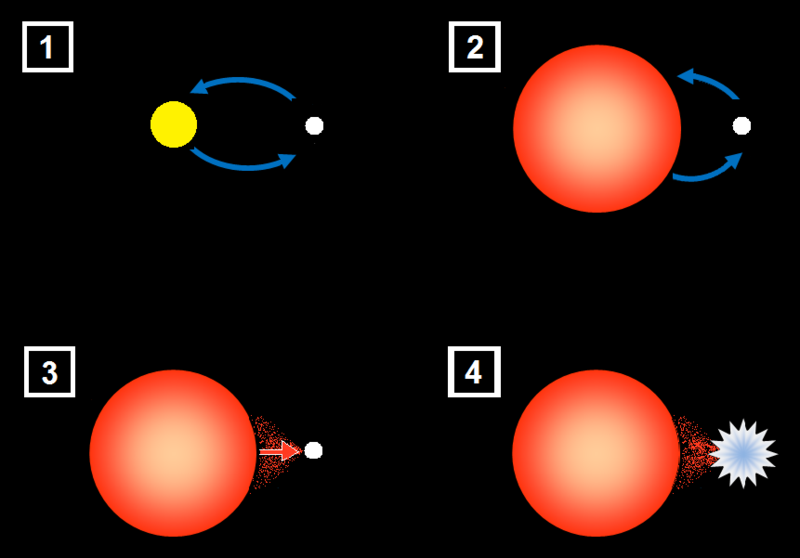
\includegraphics[width=0.4\textwidth]{SN_types.png}
          \caption{Typical luminosity-time curve for a SNIa. \newline \hfill Image: Wikipedia-author FT2}
        \end{figure}
        \begin{figure}
          \label{supcurv}
          \centering
          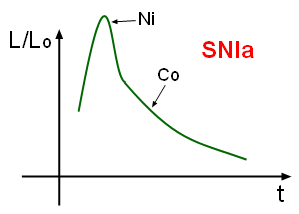
\includegraphics[width=0.4\textwidth]{SNIacurva.png}
          \caption{Typical luminosity-time curve for a SNIa. \newline \hfill Image: Wikipedia, claimed as open source (https://commons.wikimedia.org/wiki/File:SNIacurva.png)}
        \end{figure}
  \section{conclusion and outlook}
    \begin{itemize}
      \item observation of SNIa's allows precise measurements of cosmological scales
      \item comparison of data and model allows to make more precise predictions about the universe (see Figure \ref{modfit})\footnote{source: \url{supernova_fit.py}}
    \end{itemize}
    \begin{figure}%[b]
      \label{modfit}
      \centering
      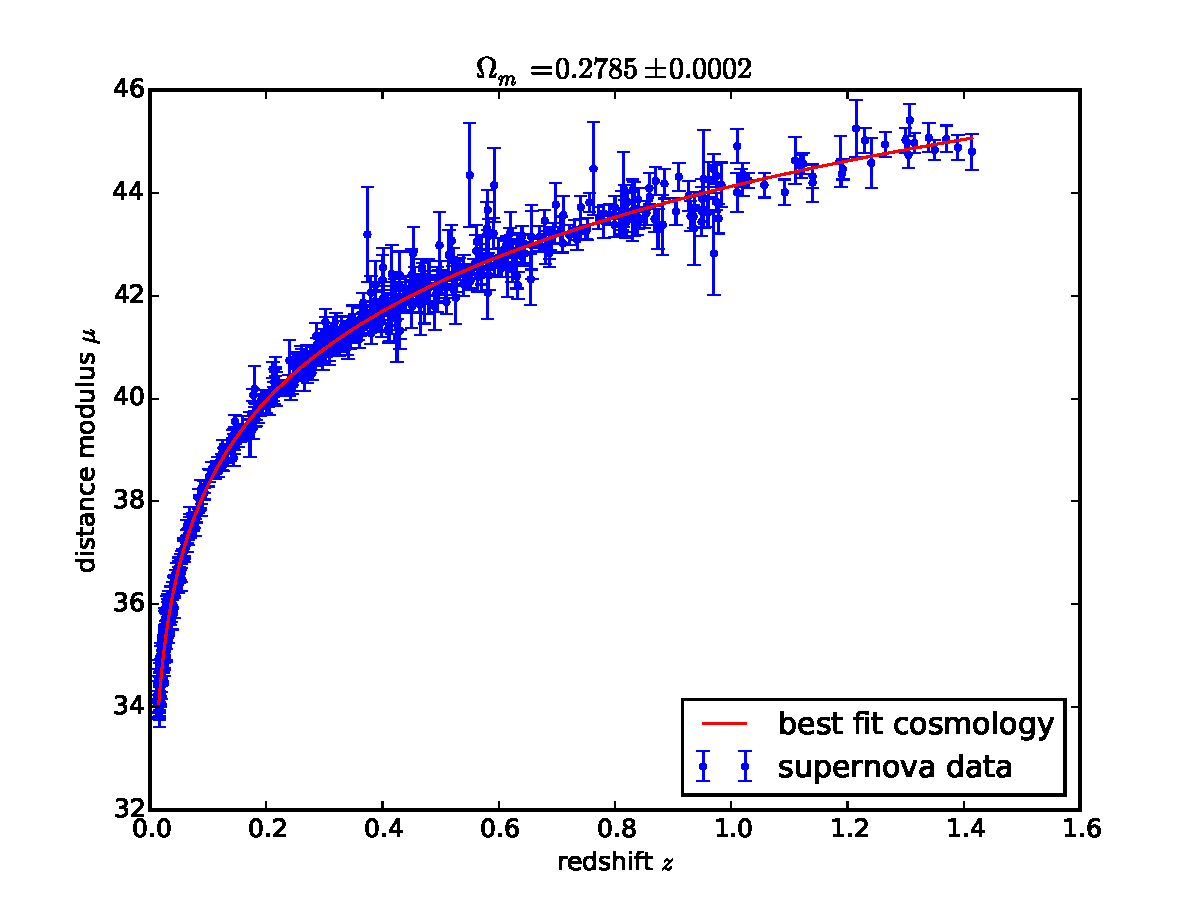
\includegraphics[width=0.8\textwidth]{supernova_fit.pdf}
      \caption{fit of a cosmological model to the measured SNIa data}
    \end{figure}
\end{document}